\documentclass[12pt,oneside,final]{article}

\usepackage{lmodern}
\usepackage{hyperref}
\usepackage{enumerate}
\usepackage{minted}
\usepackage{graphicx}

\graphicspath{{./img/}}

\begin{document}

% \input{header_page}

\let\bf\textbf
\let\it\textit

% Copyright (C) Olivier Dion \it{olivier.dion@polymtl.ca}                                                                      
% This program is free software: you can redistribute it and/or modify  
% it under the terms of the GNU General Public License as published by  
% the Free Software Foundation, either version 3 of the License, or     
% (at your option) any later version.                                   
% 
% This program is distributed in the hope that it will be useful,       
% but WITHOUT ANY WARRANTY; without even the implied warranty of        
% MERCHANTABILITY or FITNESS FOR A PARTICULAR PURPOSE.  See the         
% GNU General Public License for more details.                          
% 
% You should have received a copy of the GNU General Public License     
% along with this program.  If not, see <http://www.gnu.org/licenses/>. 


\newpage
\section{Définitions}
Avant de commencer, voyons quelques définitions.

\paragraph{Linux} ~ \\ Lorsque l'on dit \bf{Linux}, on fait référence en fait
au système d'exploitation (OS) \bf{GNU/Linux}. \it{Linux} est en fait
le noyau du système d'exploitation (\it{Kernel}). \it{Linux} (Kernel)
n'offre aucun logiciel pour l'utilisateur (\bf{userland}) par lui
même. Le \it{kernel} offre seulement ce qu'on appelle des \bf{system
  call} (\bf{syscall}), qui sont des portes d'entrées vers des
services offerts par le \it{kernel}. Pour raison de brièveté,
lorsqu'il est écrit \it{Linux} dans ce documment, et ce à partir de
maintenant, on fait référence à \it{GNU/Linux}. Lorsque l'on voudra
faire référence au \it{kernel}, on en fera explicitement la remarque.

\paragraph{GNU} ~ \\ \it{GNU} est un accronyme récursif qui veut dire \bf{GNU
  is Not Unix}. \it{GNU} est en fait un long projet (35 ans le 27
septembre) qui a pour but principal de faire un OS libre d'utilisation
visant à remplacer \bf{UNIX}. Je ne vais pas tarder sur le sujet, mais
je vous invite fortement à en lire plus \url{https://www.gnu.org/gnu/thegnuproject.en.html}.

\paragraph{GNU/Linux} ~ \\ \it{GNU/Linux} est ce que vous utilisez au
laboratoire. Vous utilisez le \it{kernel Linux} et vous utiliez comme
\it{userland GNU}.


\paragraph{Distribution} ~ \\ Il est existe des centaines de
distribution pour \it{Linux}. Une distribution est en fait un OS, basé
sur \it{GNU/Linux} qui a une collection de \it{software}
pré-installé. Une distribution a aussi ce que l'on appelle un
\bf{package manager}, qui s'assure, entre autre, de règler les
conflits de dépendances entre les logiciels,
installation/désintallation et des mises à jours de différents
logiciels ou même le \it{kernel}. Chaque distribution a sa propre
philosophie et son propre modèle de management des
\it{packages}. Voici une liste non-exhaustive de distribution et une
courte description pour chaque distribution.



\newpage \section{Distributions}

\paragraph{Ubuntu} ~ \\
Distribution probablement la plus poppulaire. Elle est très facile
d'utilisation. Basée sur la distributon \bf{Debian}, elle utilise
donc le \it{package manager} \bf{dpkg}. Utilise \bf{GNOME3} ou
\bf{Ubuntu Unity} comme interface graphique par
défaut. \bf{Attention}, avant la version \bf{16.04}, \it{Ubuntu}
espionnait ses utilisateurs en vendant des informations à des
troisièmes parties (comme Windows fait avec Cortana...). Ceci est en
passant, la définition même d'un \it{spyware}. Vous pouvez lire à ce
sujet:
\url{https://www.gnu.org/philosophy/ubuntu-spyware.en.html}. \it{Ubuntu}
est développé par la compagnie \bf{Canonical}.


\paragraph{ElementaryOS} ~ \\
Distribution concentrée sur l'expérience utilisateur. Elle est basée
sur \it{Ubuntu} et donc utilise \it{dpkg} comme \it{package
  manager}. L'interface graphique par défaut est \bf{Pantheon} qui
est sensiblement pareille que \bf{Mac OS X}. Elle est donc très
facile d'utilisation et est très jolie.


\paragraph{Solus} ~ \\
\it{Solus} est une nouvelle distribution (seulement 2 ans!) basée sur
aucune autre distribution. Elle utilise comme \it{package manager}
\bf{eopkg}. Ce qui est intéressant avec \it{Solus}, c'est qu'il
s'agit d'une \bf{Rolling} distribution. Sans rentrer dans les
détails, avec une distribution qui suit le modèle \it{rolling}, vous
aurez toujours les dernières versions de vos logiciels, \bf{driver}
(\it{e.g} carte graphique), \it{kernel}, etc. Cela est aussi à
double tranchant, vous aurez parfois des bugs dans vos logiciels car
vous êtes en quelque sorte les premiers à tester la nouvelle mise à
jour, mais cela est très rare et très vite corrigée. \it{Unbuntu} et
\it{ElementaryOS} ne sont pas des \it{rolling} distribution, alors
vous devez attendre quelque temps avant d'avoir de nouvelles mises à
jour. Enfin, \it{Solus} a par défaut comme interface graphique soit,
\bf{Budgie}, \bf{GNOME3} ou \bf{MATE}. \it{Budgie} est fait maison
par les développeurs de \it{Solus} et est très bon (quoi que j'ai eu
quelques problèmes avec...).

\paragraph{Fedora} ~ \\
C'est la distribution qu'on a dans nos laboratoires à l'école. Je ne
l'ai jamais utilisée alors je vais simplement dire qu'elle est
développée par le projet \it{Fedora} qui est sponsarisé par la
compagnie \bf{Red Hat}.


\paragraph{Arch} ~ \\
\it{Arch} est une distribution pour les utilisatrices avancées
seulement. Cette distribution est pour les processeurs à
architecture \bf{x86-64} seulement (des ports non officiels pour
\bf{i686} et \bf{ARM} existent). Elle utilise comme \it{package
  manager} \bf{pacman} et est une \it{rolling} distribution. Elle
n'utilise aucun interface graphique par défaut (mode console). La
philosophie de \it{Arch} est d'installer le strict
minimum. Contrairement à d'autre distro qui installe pleins de truc
innutile comme \it{Windows} (\it{Ubuntu} installe une application de
Amazon par défault...), \it{Arch} installe le strict minimum (kernel
+ quelques autres trucs) et rien d'autre. Vous devez donc vous même,
configurer votre \it{kernel} pour activer des services que vous
voulez (internet en autre...), installer un environnement graphique,
etc. L'avantage? Vous avez le contrôle totale sur votre
distribution. \it{Arch} possède sont propre \it{Wiki} qui documente
très bien plusieurs sujets.


\newpage \section{File System (fs)} ~ \\
Sous \it{Linux}, les fichiers sont structurés dans un arbre. La racine
de l'arbre est \bf{/}. Pour accéder par exemple à mon dossier
document, le chemin d'accès absolu est
\path{/home/olivier/Documents}. Il n'y à pas de \bf{C:} ou \bf{D:} pour
différencier les disques durs physiques comme sous \it{Window}. À la
place, le \bf{fs} va faire des points de montage virtuels à partir de
la racine. Par exemple, si je veux monter un disque dur contenant ma
musique et des films, je vais créer un dossier nommé \path{~/Media} et
je vais monter le disque à ce point. Ici, \path{~} signifie mon
répertoire maison (\path{/home/olivier} sur mon ordie). Voici un exemple
complet.

\begin{minted}{bash}
  $ mkdir ~/Media
  $ sudo mount /dev/sda ~/Media
\end{minted}

Ici, on a créé le dossier Media dans le dossier \path{~} et on a monté
le disque dur A dans le dossier \path{~/Media}.

\section{Process} À COMPLETER

\section{Variable d'environnement} Chaque \it{process}
possède une liste de variable d'environnement. Il s'agit d'une liste
de pair \bf{key:value}. Un \it{process} peut modifier à tout moment sa
liste. Lorsqu'un \it{process} est créé, celui-ci copie la liste
d'environnement de son parent.

\begin{minted}{bash}
  # Pour voir la liste d'environnement d'un shell
  $ printenv  
\end{minted}

\newpage \section{Shell \& Terminal} ~ \\

\subsection{Terminal}
Sans trop rentrer dans les détails, lorsque vous ouvrez un terminal
sous \it{Linux}, il s'agit d'un programme qui émule un vrai
terminal. Le terminal effectue une communication entre le programme
qui le contrôle et un \bf{device}. Par exemple, mon terminal à la
maison est connecté au \it{device} \path{/dev/pts/0} qui est un pseudo
terminal. Le vrai terminal de la session c'est le serveur \bf{XWindow}
(interface graphique) qui est connecté à \path{/dev/tty7}. C'est
correct si vous ne comprenez pas trop, l'important est de se rappeler
qu'un terminal est seulement là pour contrôler les inputs/outputs. Il
ne regarde pas si vous avez entrer la commande \bf{ls} par exemple.

\subsection{Shell} 
Un \it{Shell} est un programme qui se connecte à un terminal ou pseudo
terminal (faisant de lui un \bf{session leader}) et qui interprète des
commandes que vous envoyez à travers le terminal. Par défaut quand
vous ouvrez un terminal, celui-ci va executer le programme se trouvant
au chemin d'accès définit dans la variable d'environnement
\bf{SHELL}. Vous pouvez changer ce comportement en configurant votre
terminal. Par exemple chez moi, mon terminal ouvre par défaut le
programme au chemin d'accèes \bf{/bin/bash}. \it{Bash} est pour
\bf{Bourne Again Shell} et est un \it{shell} développé par
\it{GNU}. Il existe d'autre \it{shell} tels que \bf{sh}, \bf{dash},
\bf{zsh}. Chaque \it{shell} possède un language de programmation qui
se ressemble, mais peut différer sur certains points.


\newpage

\section{Bash}
Par défaut, \it{Bash} se place dans le chemin d'accès contenue dans la
variable d'environnement \bf{HOME}. Si cette variable n'existe pas ou
bien que le chemin d'accès est inexistant ou que vous n'avez pas les
droits d'accès, \it{Bash} va soit créer le dossier pour vous, ou vous
placer dans \path{~}. \it{Bash} afficher votre nom d'utilisateur
suivit du nom de l'\it{host}, le chemin d'accès dans lequel vous vous
trouvez et dans quel mode vous vous
trouvez. Voici une capture d'écran pour vous montrer. \\

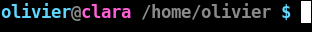
\includegraphics[scale=2]{bash_1} \\


\bf{olivier} est mon nom d'utilisateur, \bf{clara} est le nom
d'\it{host} de mon ordinateur. Je me trouve dans le répertoire
\path{/home/olivier} et je suis en mode utilisateur normal \bf{\$}. Si
je veux aller en mode administrateur (\bf{root}), je peux faire la
commande \bf{sudo su}. Ne le faite pas sur les poste à l'école! \\

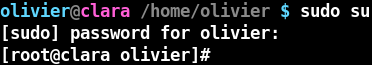
\includegraphics[scale=2]{bash_2} \\

Comme vous pouvez le voir, sur \it{Linux} la sécurité est très
importante. Et donc, lorsque l'on demande mon mot de passe, on n'affiche
rien, même pas de \bf{*****}. Comme ça, vous ne pouvez pas savoir la
longueur de mon mot de passe! De plus, le \bf{\$} a été remplacé par
\bf{\#} car je suis maintenant connecté en tant que \bf{root}.

\newpage
\subsection{Lister les fichiers}
Avant de nous déplacer, commençon par lister le dossier dans lequel on
se trouve. \\

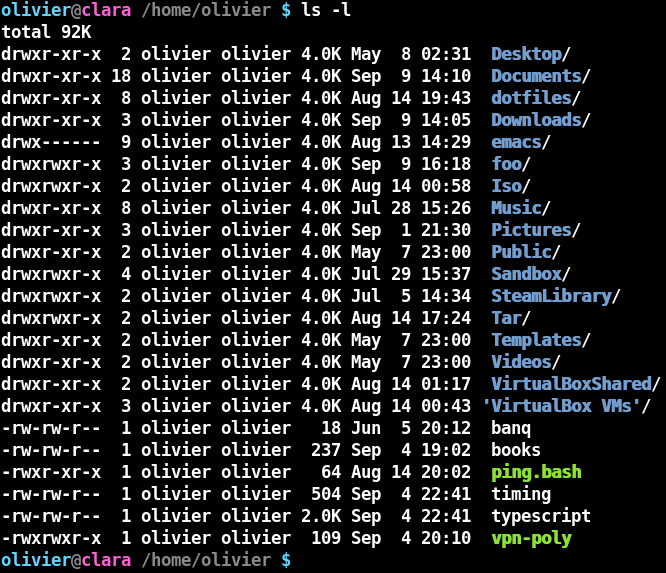
\includegraphics[scale=2]{bash_ls} \\

La dernière colonne est le nom des fichiers dans le dossier
courrant. Ici, j'ai customisé mon \it{shell} pour lister les dossiers
en bleu, les fichiers ordinaires en blanc et les exécutables en
vert. La première colonne représente les permissions d'accès au
fichier. \bf{d} veut dire \it{directory}. \bf{r} veut dire \it{read},
\bf{w} write et \bf{x} \it{execute}. Un \bf{-} veut dire aucune
permission. Les permissions sont répéter 3 fois. La première fois pour
l'utilisateur a qui appartient le fichier, la deuxième fois pour le
groupe auquel le fichier appartient et enfin le dernier pour les
autres utilisateurs. La deuxième colonne représente le nombre de lien
vers le fichier. La troisième et quatrième colonne représentent
respectivement l'utilisateur et le groupe propriétaire du fichier. La
cinquième colonne donne la taille du fichier en octet. Enfin, de la
sixième à la huitième colonne, il s'agit du \it{timestamp} du fichier. \\

Par exemple, le fichier \bf{banq} est un fichier ordinaire
(\bf{-}). L'utilisateur et le groupe propriétaire ont le droit de lire
et d'éditer le fichier \bf{rw-} et les autres utilisateurs ont
seulement le droit de le lire \bf{r--}. Le propriétaire du fichier est
\bf{olivier} et le groupe propriétaire est \bf{olivier}. Le fichier
pèse 18 octets et a été modifié la dernière fois le 5 Juin à 20:12. \\


Les fichiers cachés non pas été lister par contre. Un fichier caché
commence par un point (\bf{.}). Pour lister les fichiers cachés, il
faut inclure dans la commande \bf{ls}
l'option \bf{-a} (\bf{all}). \\

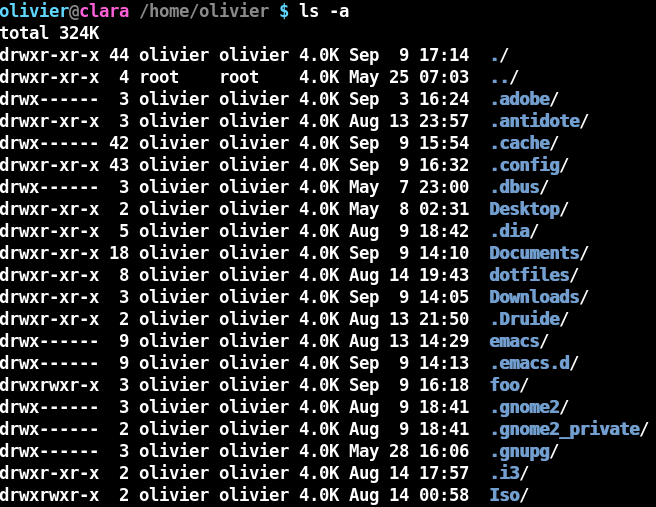
\includegraphics[scale=2]{bash_ls_2} \\

On voit qu'il y avait beaucoup de fichiers cachés (la liste continue
encore en bas). Vous remarquerez aussi les deux fichiers spéciaux
\bf{.} et \bf{..}. \bf{.} signifie le répertoire courrant tandit que
\bf{..} est le répertoire parent. Donc, dans \path{/home/olivier},
\bf{..} représente \path{/home} et \bf{.} \path{/home/olivier}. Enfin,
pour afficher tous les fichiers sauf \bf{.} et \bf{..}, utiliser
l'option \bf{-A} (\bf{Almost all}).

\newpage
\subsubsection{Chemin d'accès absolu et relafif}
Un chemin d'accès absolu commence toujours par la racine. Un chemin
d'accès relatif commence soit par \bf{.} ou bien \bf{..}. Par exemple, \\
\path{/usr/include/SDL2/SDL_vulkan.h} est un chemin absolu tandit que \\
\path{../Documents/Poly/LOG1000/README} et \\
\path{./patrick_watson/close_to_paradise/the_great_escape.mp3} sont
des chemins relatifs. Dans certain cas, \it{Bash} va interpréter un
chemin ne remplissant aucune des conditions précédentes comme un
chemin relatif au dossier courrant. Par exemple, \\
\path{Dossiers/Poly} va être vue comme \path {~/Dossiers/Poly} si je
suis dans \path{~}.

\newpage
\section{Se Promener}
La commande \bf{cd} (\bf{Change Directory}) permet de changer de
répertoire courrant. On peut soit passer un chemin absolu ou bien un
chemin relatif. Si aucun chemin n'est spécifié, \it{Bash} retourne à
\bf{HOME}. On peut aussi retourner au dernier dossier visité à l'aide
de \bf{cd -}. \\

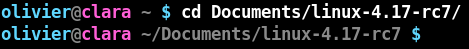
\includegraphics[scale=2]{bash_cd} \\


\section{Supprimer}
Pour supprimer des fichiers, on utilise la commande \bf{rm}
(\bf{remove}). \bf{Attention}, cela ne place pas les fichiers dans la
corbeille. Ceux-ci sont perdus à jamais (ou presque). Pour supprimer
un dossier (et donc les fichiers dans le dossier), on doit passer
l'option \bf{-r} (\bf{recursive}) à la commande. \\

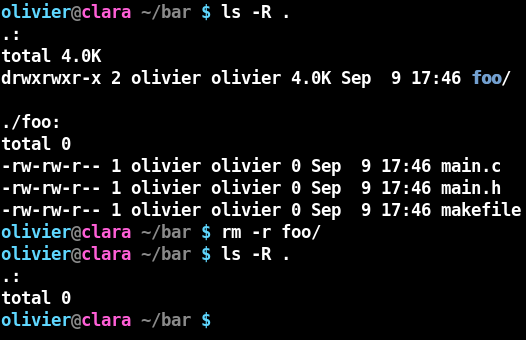
\includegraphics[scale=2]{bash_rm} \\


\newpage
\section{Grep}
La commande \bf{grep} est un outil extrêmement puissant qui vous
permet de chercher une expression dans des fichiers. \bf{grep} (la
version de \it{GNU}) accepte aussi les expressions régulières. \\

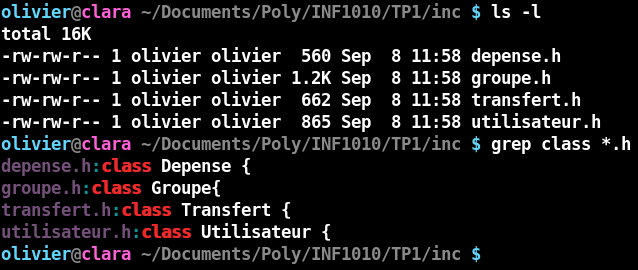
\includegraphics[scale=2]{grep} \\


\section{Sed}
À COMPLETER
\section{Awk}
À COMPLETER
\section{GCC}
À COMPLETER
\section{Emacs}
À COMPLETER


\newpage
\section{Manuel}
La commande \bf{man} vous permet de lire le manuel d'une commande,
d'un programme, d'un syscall, etc. \bf{man} est divisé en 7 sections.

\begin{enumerate}[1]
\item Commandes générales
\item Syscall
\item Fonctions de libraries
\item Fichiers spéciaux
\item Formats de fichiers
\item Jeux
\item Autres
\item Administration du système
\end{enumerate}

Par exemple, si vous voulez lire sur \bf{write}. Il existe
\bf{write(1)}, mais aussi \bf{write(2)}. Par défaut, \bf{man} va
ouvrir la première page du manuel quelle trouve (\bf{write(1)}). Si
vous voulez lire \bf{write(2)}, vous devez spécifier 2 comme argument.

\begin{minted}{bash}
  $ man write   # Va ouvrir write(1)
  ...
  $ man 2 write # Va ouvrir write(2)
\end{minted}

Vous pouvez ainsi lire le manuel des commandes parlées précédament,
par exemples \bf{man ls} ou bien \bf{man grep}. Vous pouvez aussi lire
le manuel de \bf{man}. \bf{man man}.


\section{Help}
Si vous êtes perdu, vous pouvez tapper la commande \bf{help} dans le
terminal. Une liste de commande sera alors affichée. Utilisé ceci avec
\bf{man} et vous devriez être correct.

\end{document}